\section{Performance}
\sectiontoc

\subsection{Theoretical Limits}
\begin{frame}{Theoretical Limits}
    \begin{quote}
        A well designed Lustre storage system can achieve
        90\% of underlining hardware bandwidth.

        \hspace*\fill{\scriptsize--- Zhiqi Tao, Sr. System Engineer, Intel \cite{10-intel}}
    \end{quote}

    \pause

    \textbf{Example}

    \begin{itemize}
        \item<+-> 160 OSS, 16 OST each, 2 TiB each (old limits)
        \item<+-> $\rightarrow$ 2.5 PiB (Pebibyte) total storage
        \item<+-> each OST delivers 50 MiB/s
        \item<+-> $\rightarrow$ 800 MiB/s combined throughput per OSS
        \item<+-> stripe size 16 MiB
        \item<+-> write 200 GiB file (80 stripes per OSS, 5 stripes per OST)
        \item<+-> $\rightarrow$ 1.25 GiB per OSS, written in 1.6 seconds
        \item<+-> all OSS parallel, total speed 125 GiB/s
    \end{itemize}
\end{frame}

\subsection{Bottlenecks}
\begin{frame}{Metadata overhead}
    \textbf{Common Task}
    \begin{itemize}
        \item directory traversal and \textbf{stat} (\texttt{ls -l})
    \end{itemize}

    \textbf{Problem}
    \begin{itemize}
        \item one \texttt{stat} call for every file, each is a RPC (POSIX).
        \item each RPC generates overhead and I/O wait
    \end{itemize}

    \textbf{Solution}
    \begin{itemize}
        \item kernel detects traversal+stat and requests all stats from OSS in advance (parallel)
        \item a combined RPC reply is sent (up to 1 MB)
    \end{itemize}
\end{frame}

\begin{frame}{Metadata overhead (cont'd)}
    \makebox[0.5\textwidth][c] {
        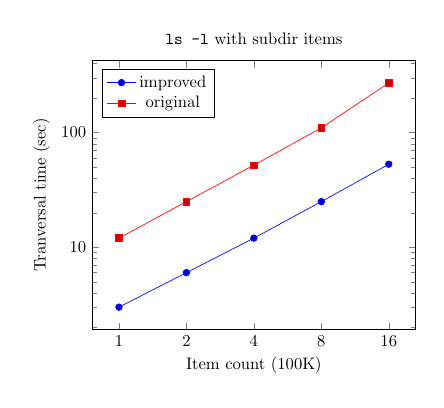
\begin{tikzpicture}[scale=0.6]
            \begin{loglogaxis}[
                xlabel={Item count (100K)},
                log basis x=2,
                xticklabel=\pgfmathparse{2^\tick}\pgfmathprintnumber{\pgfmathresult},
                ylabel={Tranversal time (sec)},
                yticklabel=\pgfmathparse{10^\tick}\pgfmathprintnumber{\pgfmathresult},
                log basis y=10,
                legend pos=north west,
                title={\texttt{ls -l} with subdir items}
                ]
                %\axispath\draw
                        %(7.49165,-10.02171)
                    %|-  (8.31801,-11.32467)
                    %node[near start,left] {$\frac{dy}{dx} = -1.58$};

                \addplot plot coordinates {
                    (1, 3)
                    (2, 6)
                    (4, 12)
                    (8, 25)
                    (16, 53)
                };
                %
                \addlegendentry{improved}

                \addplot plot coordinates {
                    (1, 12)
                    (2, 25)
                    (4, 52)
                    (8, 110)
                    (16, 271)
                };
                \addlegendentry{original}
            \end{loglogaxis}
        \end{tikzpicture}
    }\makebox[0.5\textwidth][c] {
        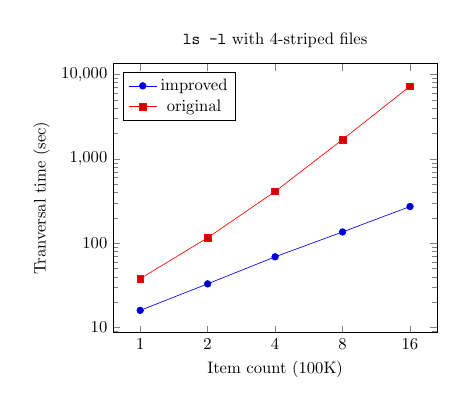
\begin{tikzpicture}[scale=0.6]
            \begin{loglogaxis}[
                xlabel={Item count (100K)},
                log basis x=2,
                xticklabel=\pgfmathparse{2^\tick}\pgfmathprintnumber{\pgfmathresult},
                ylabel={Tranversal time (sec)},
                yticklabel=\pgfmathparse{10^\tick}\pgfmathprintnumber{\pgfmathresult},
                log basis y=10,
                legend pos=north west,
                title={\texttt{ls -l} with 4-striped files},
                ]
                %\axispath\draw
                        %(7.49165,-10.02171)
                    %|-  (8.31801,-11.32467)
                    %node[near start,left] {$\frac{dy}{dx} = -1.58$};

                \addplot plot coordinates {
                    (1, 16)
                    (2, 33)
                    (4, 69)
                    (8, 136)
                    (16, 272)
                };
                \addlegendentry{improved}

                \addplot plot coordinates {
                    (1, 38)
                    (2, 116)
                    (4, 410)
                    (8, 1692)
                    (16, 7248)
                };
                \addlegendentry{original}
            \end{loglogaxis}
        \end{tikzpicture}
    }

    \vspace{1cm}
    \hfill{\scriptsize\emph{graph data from \cite{metadata-scaling}}}
\end{frame}

\subsection{Improvements}
\begin{frame}{Improvements}
    \textbf{Recently implemented}
    \begin{itemize}
        \item OSS/file limit extended (wide striping, $> 160$ OSS possible)
    \end{itemize}

    \textbf{Planned features}
    \begin{itemize}
        \item ZFS instead of ldiskfs
        \item metadata striping / namespacing (multiple MDS)
    \end{itemize}
\end{frame}

\subsection{Scalability}
\begin{frame}{Scalability}
    \begin{itemize}
        \item Lustre distributes bandwidth evenly over OSS (striping)
        \item different network types simultaneously (InfiniBand, TCP: GigE)
        \item more OSS can always be added (for more bandwidth and/or capacity)
        \item current bottleneck: MDS
    \end{itemize}
\end{frame}
